% 
% topic Template for ME3050 -  Dynamics Modeling and Controls - Tennessee Technological University
%
% Lecture Template for ME3050-001-002-Tristan Hill - Spring 2020 - Summer
% Dynamics Modeling and Controls
% Module 2 - Dynamics Review 
% Topic 1 - Describing Motion 

% Document settings

%\documentclass{beamer}                  % for presentation ?
\documentclass[handout]{beamer}  % for handout ?
\usepackage{beamerthemesplit}
\usepackage{amsmath}
\usepackage{listings}
\usepackage{multicol}
\usepackage{framed}
\usepackage{amsmath, nccmath}
\usepackage{geometry}
\usepackage{bm}

\beamertemplateballitem

\definecolor{TTUpurple}{rgb}{0.3098, 0.1607, 0.5176} % TTU Purple (primary)
\definecolor{TTUgold}{rgb}{1.0000, 0.8666, 0.0000} % TTU Gold (primary)

\setbeamercolor{palette primary}{bg=TTUpurple,fg=TTUgold}
\setbeamercolor{palette secondary}{bg=black,fg=TTUgold}
\setbeamercolor{palette tertiary}{bg=black,fg=TTUpurple}
\setbeamercolor{palette quaternary}{bg=TTUgold,fg=black}
\setbeamercolor{structure}{fg=TTUpurple} % itemize, enumerate, etc
\setbeamercolor{section in toc}{fg=TTUpurple} % TOC sections

% custom colors
\definecolor{TTUpurple}{rgb}{0.3098, 0.1607, 0.5176} % TTU Purple (primary)
\definecolor{TTUgold}{rgb}{1.0000, 0.8666, 0.0000} % TTU Gold (primary) 
\definecolor{mygray}{rgb}{.6, .6, .6}
\definecolor{mypurple}{rgb}{0.6,0.1961,0.8}
\definecolor{mybrown}{rgb}{0.5451,0.2706,0.0745}
\definecolor{mygreen}{rgb}{0, .39, 0}
\definecolor{mypink}{rgb}{0.9960, 0, 0.9960}

% color commands
\newcommand{\R}{\color{red}}
\newcommand{\B}{\color{blue}}
\newcommand{\BR}{\color{mybrown}}
\newcommand{\K}{\color{black}}
\newcommand{\G}{\color{mygreen}}
\newcommand{\PR}{\color{mypurple}}
\newcommand{\PN}{\color{mypink}}
\newcommand{\OR}{\color{orange}}
\newcommand{\GD}{\color{TTUgold}}


\newcommand{\Lagr}{\mathcal{L}} % lagrangian

\newcommand{\hspcu}{\underline{\hspace{20mm}}} % large horizontal space w underline
\newcommand{\vspccc}{\vspace{6mm}\\} % large vertical space
\newcommand{\vspcc}{\vspace{4mm}\\}   % medium vertical space
\newcommand{\vspc}{\vspace{2mm}\\}     % small vertical space

\newcommand{\hspcccc}{\hspace{10mm}} % large horizontal space
\newcommand{\hspccc}{\hspace{6mm}} % large horizontal space
\newcommand{\hspcc}{\hspace{4mm}}   % medium horizontal space
\newcommand{\hspc}{\hspace{2mm}}     % small horizontal space

\newsavebox{\mybox} % custom box

\newcommand{\MNUM}{2\hspace{2mm}} % Module number
\newcommand{\TNUM}{1\hspace{2mm}} % Topic number 
\newcommand{\moduletitle}{Dynamics Review} % Titles and Stuff
\newcommand{\topictitle}{Describing Motion} 

\newcommand{\sectiontitleI}{Translation} % More Titles and Stuff
\newcommand{\sectiontitleII}{Rotation}
\newcommand{\sectiontitleIII}{Equations of Rotations}
\newcommand{\sectiontitleIV}{Degrees of Freedom}
\newcommand{\sectiontitleV}{DOF Examples}


\author{ME3050 - Dynamic Modeling and Controls}
\title{Module \MNUM - \moduletitle}
\date{Mechanical Engineering\vspc Tennessee Technological University}

\begin{document}

\lstset{language=MATLAB,basicstyle=\ttfamily\small,showstringspaces=false}

\frame{\titlepage \center\begin{framed}\Large \textbf{Topic \TNUM - \topictitle}\end{framed} \vspace{5mm}}

% Section 0 - Outline
\frame{
	
	\large \textbf{Topic \TNUM - \topictitle} \vspace{3mm}\\
	
	\begin{itemize}
	
		\item \sectiontitleI    \vspc % Section I
		\item \sectiontitleII 	\vspc % Section II
		\item \sectiontitleIII 	\vspc %Section III
		\item \sectiontitleIV 	\vspc %Section IV
		%\item \sectiontitleV 	\vspc %Section V
	
	\end{itemize}

}

% Section 1:

\section{Translation}

\frame{
\frametitle{Translation}

\begin{multicols}{2}
Translational motion is: \vspc
\begin{itemize}
\item motion along a straight line.
\item rotation about a point far away? \vspace{3mm}
\end{itemize}
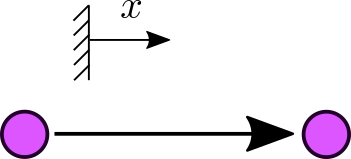
\includegraphics[scale=0.5]{translation.png}
\end{multicols}

\renewcommand{\arraystretch}{1.5}
\begin{tabular}{|l|l|} \hline
Position&$x(t)$\\ \hline
Velocity&$v_x(t)=\frac{dx(t)}{dt}=\dot{x}$\\ \hline
Acceleration&$a_x(t)=\frac{dv(t)}{dt}=\frac{d^2x(t)}{dt^2}=\ddot{x}$ \\ \hline
\end{tabular}

}

% Section 2: 
\section{Rotation}

\frame{
\frametitle{Rotation}

\begin{multicols}{2}
Rotational motion is: \vspc
\begin{itemize}
\item motion along a circular path about a fixed point or axis
\item acceleration towards the center of rotation  \vspace{3mm}
\end{itemize}

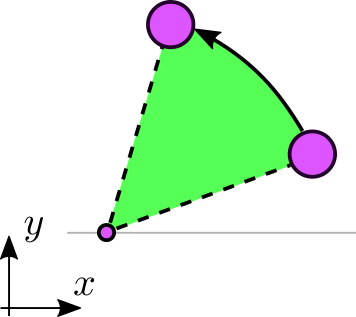
\includegraphics[scale=0.4]{rotation.png}
\end{multicols}

\renewcommand{\arraystretch}{1.5}
\begin{tabular}{|l|l|} \hline
Angular Position&$\theta_z(t)$\\ \hline
Angular Velocity&$\omega_z(t)=\frac{d\theta(t)}{dt}=\dot{\theta}$\\ \hline
Angular Acceleration&$\alpha_z(t)=\frac{d\omega(t)}{dt}=\frac{d^2\theta(t)}{dt^2}=\ddot{\theta}$ \\ \hline
\end{tabular}

}

\section{Equations of Rotation}

\frame{
\frametitle{Equations of Rotation}

You used these important relationships in your dynamics course. \vspcc

\scalebox{1}{$\vec{v}=\vec{r}\times\vec{\omega}$} 

With the planar motion assumption this vector equation can be reduced to scalar equation. \vspc

\scalebox{1}{$v=r\omega$}

}

%Section 3:
\section{Degrees of Freedom}

\frame{
\frametitle{Degrees of Freedom}

The Degrees of Freedom is the number of independent motions that exist in a system. \vspc

OR \vspc

The Degrees of Freedom is the minimum number of coordinates required to completely describe motion or state of the system.


}

%Section 4:
\section{DOF Examples}

\frame{
\frametitle{DOF Examples}

Find the degrees of freedom for each of the following systems. \vspcc

\scalebox{.7}{Wittener Metronome \hspace{10mm}Passenger Aircraft \hspace{10mm} Ackermann Steeting Mechanism} \vspc
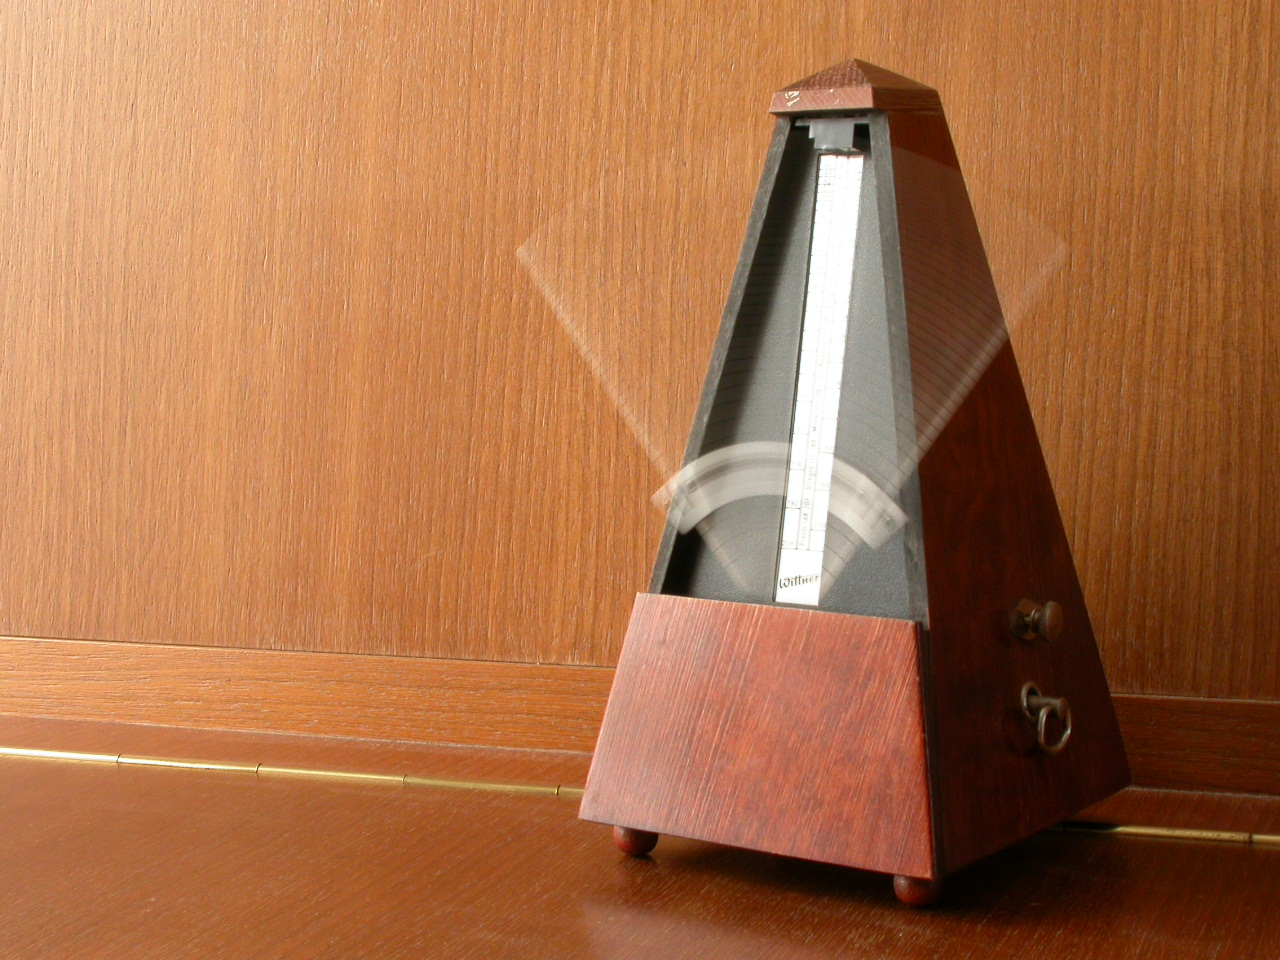
\includegraphics[scale=.25]{Wittner_metronome.jpg} \hspc 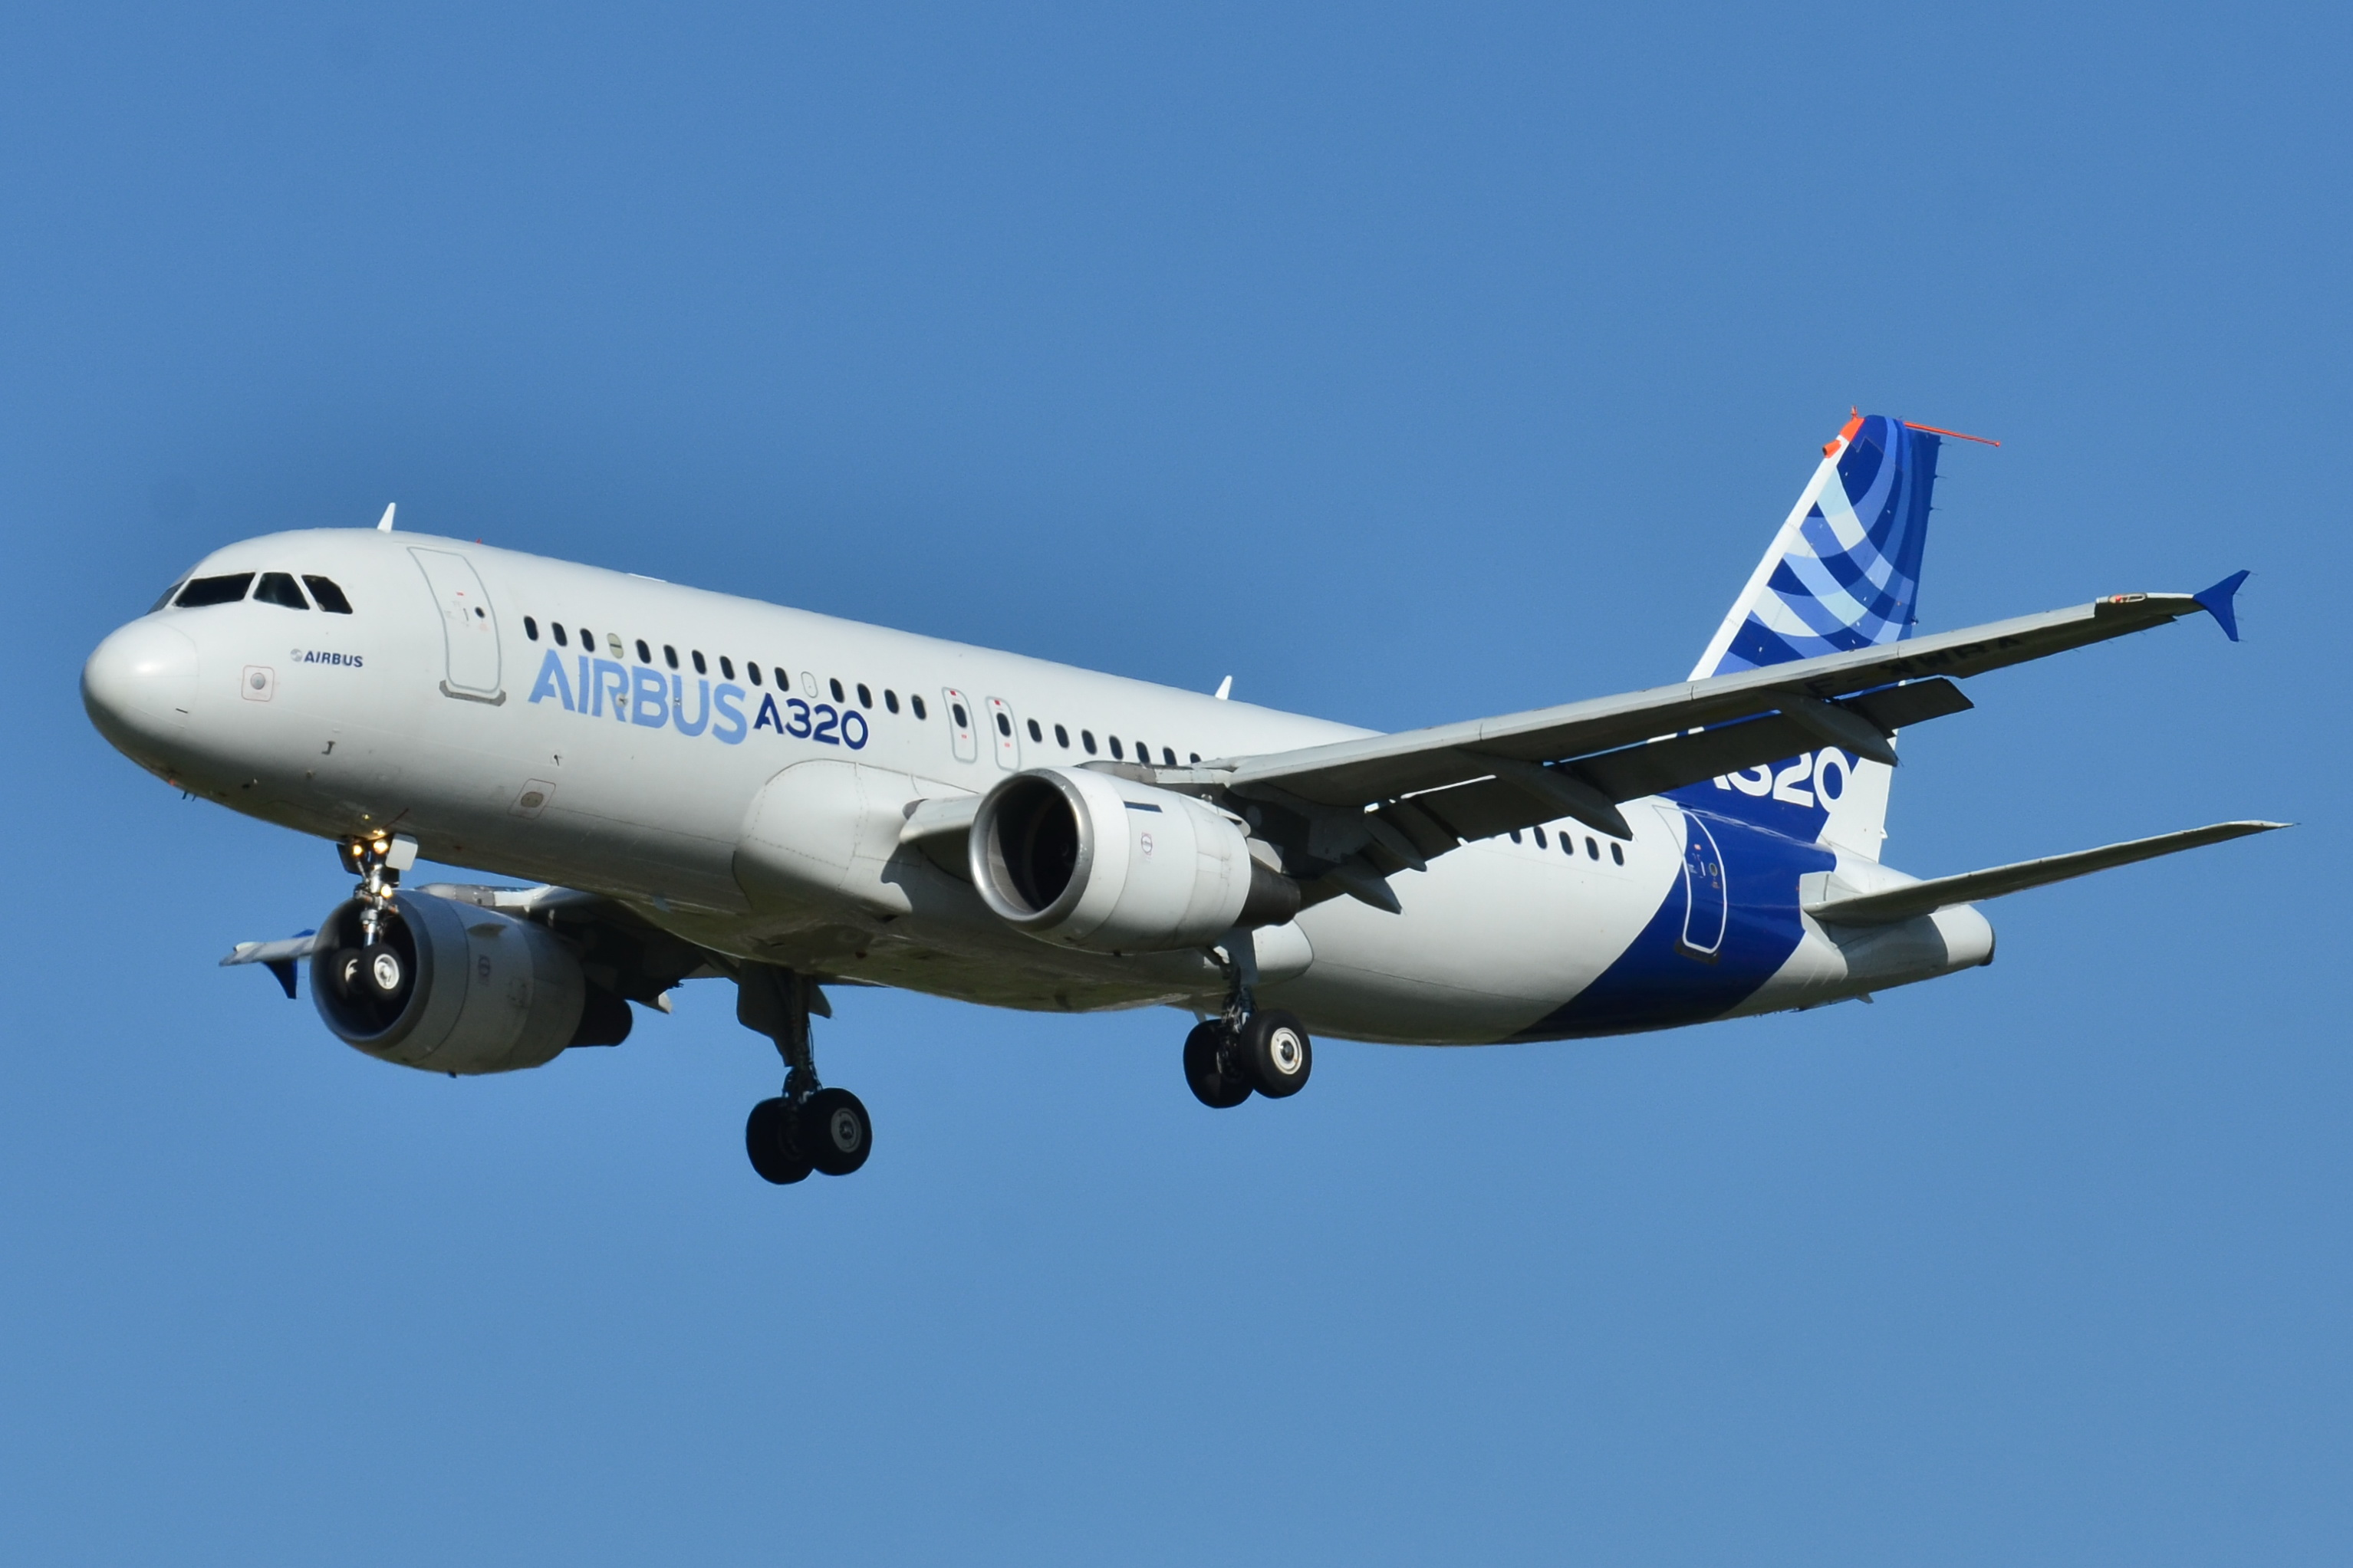
\includegraphics[scale=.125]{airbus_a320.jpg} \hspc 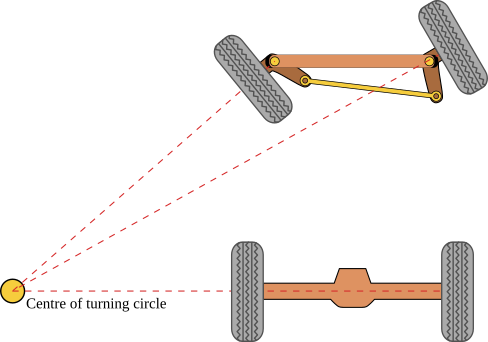
\includegraphics[scale=.25]{Ackermann_turning.png}

{\tiny \href{https://en.wikipedia.org/wiki/Metronome}{Image: Wikipedia}  \hspace{20mm}\href{https://en.wikipedia.org/wiki/Airliner}{Image: Wikipedia} \hspace{20mm}\href{https://en.wikipedia.org/wiki/Ackermann_steering_geometry}{Image: Wikipedia} }
}	
	
\end{document}



